%% The "\appendix" call has already been made in the declaration
%% of the "appendices" environment (see thesis.tex).
\chapter{Miscellanious}
\section{Intersection Tester Doxygen Sample} \label{app:Pointless}
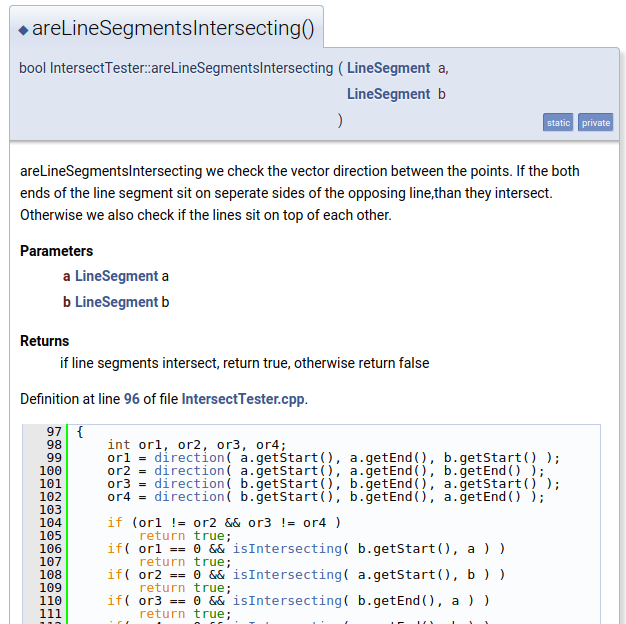
\includegraphics[width=1\textwidth]{images/softwareDevelopment}


\section{Table of Data}
We add a table of data with some useful websites that are used during the process of the thesis. \\ ~ \\
%\begin{table}
\begin{scriptsize}
\begin{tabularx}{1\textwidth}{|c|X|r|} \hline
Name & Description & Reference \\ \hline
\multicolumn{3}{|c|}{\textbf{Shapefiles}} \\ \hline
GADM & GADM holds a large selection of Shape Files for countries across the world. It was always the first place I looked when reviewing potential shape files. (Germany, Italy, Brazil, UK, Japan, etc.) \newline \url{http://www.gadm.org/country} & \cite{GAA} \\ \hline
Texas & Shapefile used to represent Texas \newline \url{https://catalog.data.gov/dataset/} & \cite{Texas} \\ \hline
Hawaii & Shapefile used to represent Hawaii \newline \url{http://planning.hawaii.gov/gis/download-gis-data/}& \cite{hawaii} \\ \hline
LSOA Wales & Extra boundaries used to represent Wales \newline \url{https://data.gov.uk/dataset/
output-areas-oa-boundaries}& \cite{wales} \\ \hline
US Counties & Counties of the United States \newline \url{http://www.census.gov/geo/maps-data/data/cbf/cbf_counties.html}& \cite{USCB} \\ \hline
\multicolumn{3}{|c|}{\textbf{Datasets}} \\ \hline
LSOA Wales& Population Data \newline \url{https://bit.ly/2hkV0a6}&\cite{ONS}\\ \hline
US Counties& Assortment of county data for the us counties \newline \url{https://
www.census.gov/library/publications/2011/compendia/usa-counties-2011.html}&\cite{USCB2}\\ \hline
Public Health England & Public Healthcare data for the CCGs of England \newline \url{https://fingertips.phe.org.uk}& \cite{publicHealthEngland}\\ \hline
Ordnance Survey Ireland& Census Data for the Republic of Ireland \newline \url{https://bit.
ly/2Dyg7Ac}&\cite{electoralDivisions}\\ \hline
\end{tabularx}
\end{scriptsize}
%\end{table}

\section{Introduction to QGIS (Guidelines for QGIS Tutorial for CGVC 2018)}
We include an appendix piece used to guide a tutorial that introduces QGIS as a useful visualization tool at the Computer Graphics and Visual Computing Conference for 2018. The tutorial aims to give an understanding of how QGIS can be used to explore two depicitions of data. Example data is provided.
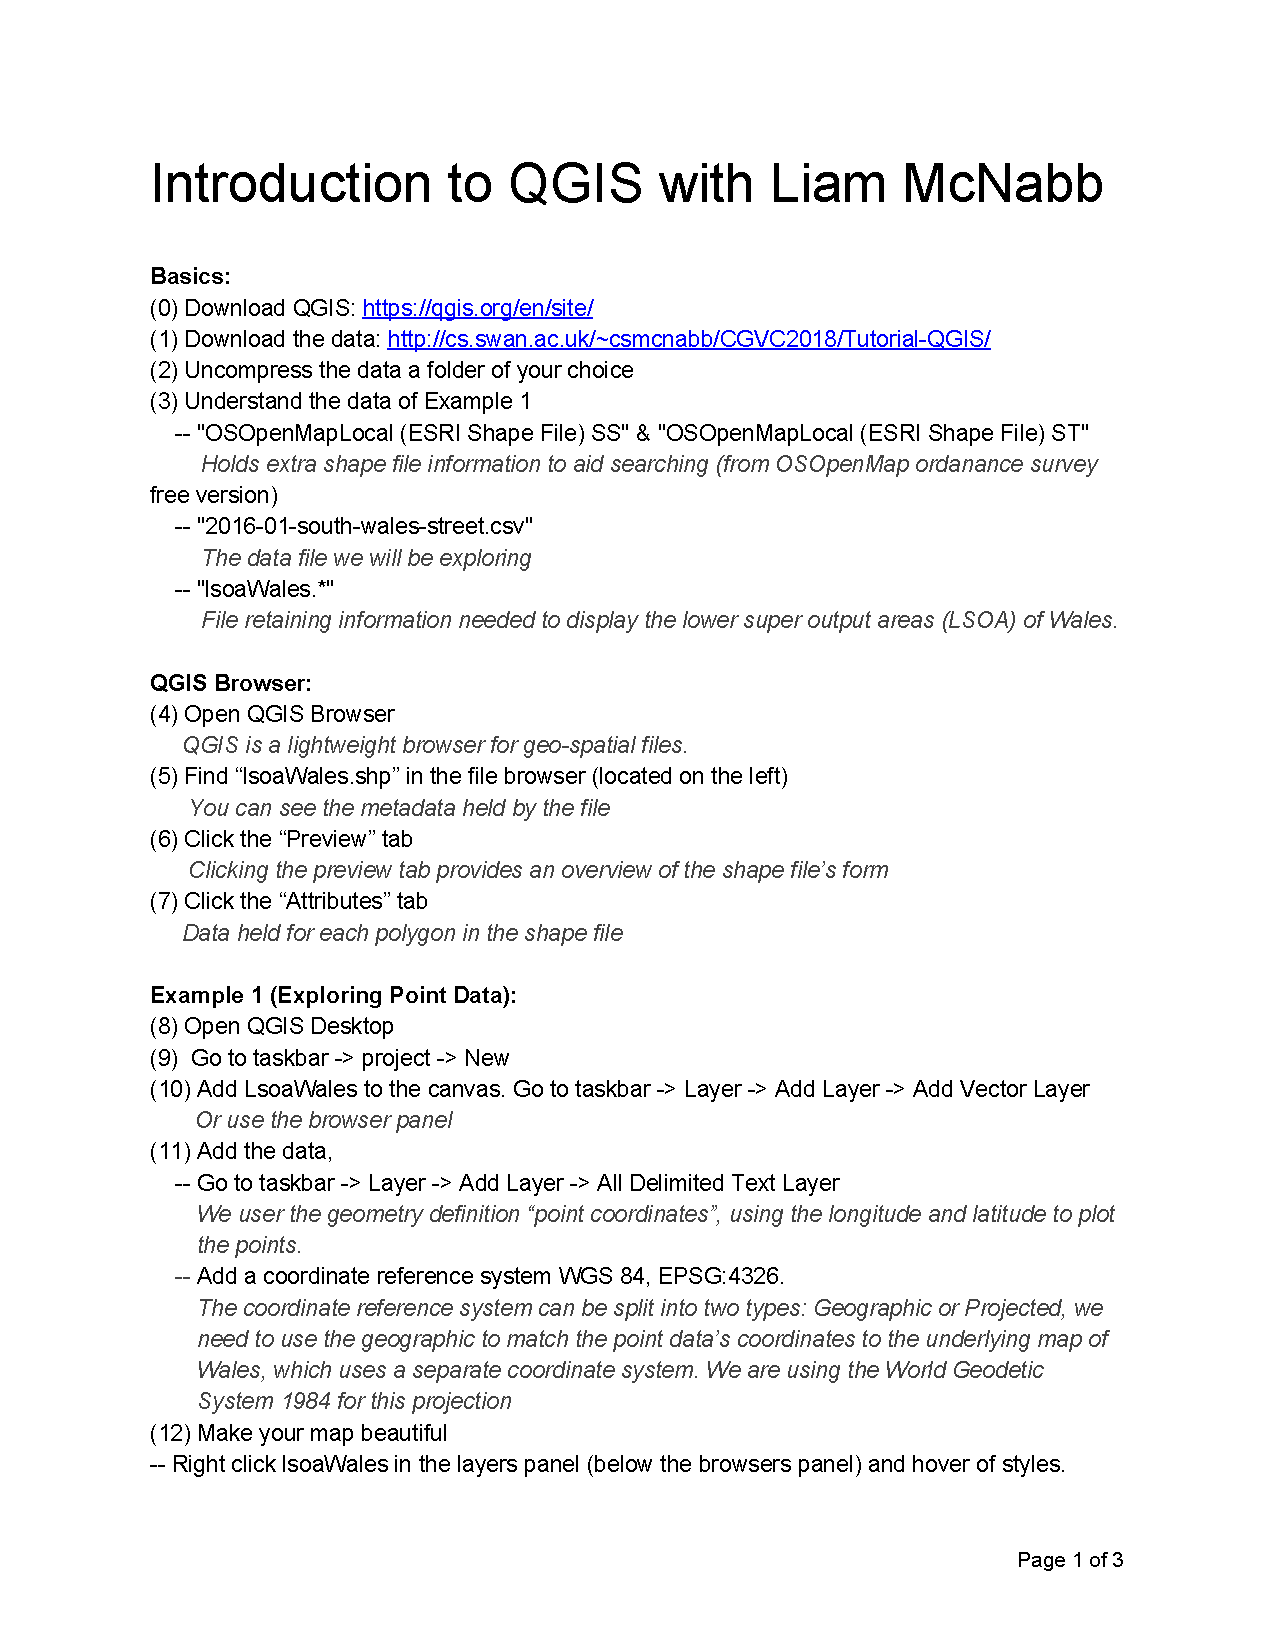
\includepdf[page={1,2,3}]{src/IntroductionToQGIS.pdf}
 
%\chapterquote{%
%Le savant n'\'etudie pas la nature parce que cela est utile; \\
%\indent il l'\'etudie parce qu'il y prend plaisir, \\
%\indent et il y prend plaisir parce qu'elle est belle.}%
%{Henri Poincar\'e, 1854--1912}

%Appendixes (or should that be ``appendices''?) make you look really clever, 'cos
%it's like you had more clever stuff to say than could be fitted into the main
%bit of your thesis. Yeah. So everyone should have at least three of them\dots
%
%\section{Like, duh}
%\label{sec:Duh}
%Padding? What do you mean?
%
%\section{$y = \alpha x^2$}
%\label{sec:EqnTitle}
%See, maths in titles automatically goes bold where it should (and check the
%table of contents: it \emph{isn't} bold there!) Check the source: nothing
%needs to be specified to make this work. Thanks to Donald Arsenau for the
%teeny hack that makes this work.

%% Big appendixes should be split off into separate files, just like chapters
%\input{app-myreallybigappendix}
